\documentclass[letterpaper]{article} % DO NOT CHANGE THIS
\usepackage[submission]{aaai2027}  % DO NOT CHANGE THIS
\usepackage[hyphens]{url}  % DO NOT CHANGE THIS
\usepackage{graphicx} % DO NOT CHANGE THIS
\urlstyle{rm} % DO NOT CHANGE THIS
\def\UrlFont{\rm}  % DO NOT CHANGE THIS
\usepackage{natbib}  % DO NOT CHANGE THIS AND DO NOT ADD ANY OPTIONS TO IT
\usepackage{caption} % DO NOT CHANGE THIS AND DO NOT ADD ANY OPTIONS TO IT
\frenchspacing  % DO NOT CHANGE THIS
\usepackage{algorithm}
\usepackage{algorithmic}
\usepackage{booktabs}
\usepackage{amsmath}
\usepackage{amsthm}
\usepackage{tikz}
\usetikzlibrary{positioning,arrows.meta}
\pdfinfo{
/TemplateVersion (2027.1)
}
% generated by make_numbers.py -- do not edit
\newcommand{\Classification}{CONDITIONAL_GO}
\newcommand{\CritCFive}{True}
\newcommand{\CritCFour}{True}
\newcommand{\CritCOne}{True}
\newcommand{\CritCSix}{False}
\newcommand{\CritCThree}{inconclusive}
\newcommand{\CritCTwo}{True}
\newcommand{\Critvalidity}{True}
\newcommand{\DevOnecritexpandVsBFiveCI}{[-0.0245, -0.0126]}
\newcommand{\DevOnecritexpandVsBFiveHolm}{3.1\cdot10^{-5}}
\newcommand{\DevOnecritexpandVsBFiveRel}{44.5}
\newcommand{\DevOnecritexpandVsBFiveSign}{-}
\newcommand{\DevOnecritexpandVsBFiveWL}{20/0}
\newcommand{\DevOnecritexpandVsBZeroCI}{[-0.0140, -0.0057]}
\newcommand{\DevOnecritexpandVsBZeroHolm}{6.0\cdot10^{-4}}
\newcommand{\DevOnecritexpandVsBZeroRel}{29.4}
\newcommand{\DevOnecritexpandVsBZeroSign}{-}
\newcommand{\DevOnecritexpandVsBZeroWL}{19/1}
\newcommand{\DevOnecritexpandVstimewindowCI}{[-0.0025, +0.0046]}
\newcommand{\DevOnecritexpandVstimewindowHolm}{1.00}
\newcommand{\DevOnecritexpandVstimewindowRel}{4.9}
\newcommand{\DevOnecritexpandVstimewindowSign}{+}
\newcommand{\DevOnecritexpandVstimewindowWL}{10/10}
\newcommand{\FigTwoOneFiveCritAt}{1.0}
\newcommand{\FigTwoOneFiveSrAt}{1.3}
\newcommand{\FigTwoOneFiveTwAt}{1.2}
\newcommand{\FigTwoTwoZeroCritAt}{1.7}
\newcommand{\FigTwoTwoZeroSrAt}{2.8}
\newcommand{\FigTwoTwoZeroTwAt}{2.0}
\newcommand{\MTwoRoundCritFeas}{376}
\newcommand{\MTwoRoundCritInfeas}{7988}
\newcommand{\MTwoRoundCritN}{82.4}
\newcommand{\MTwoRoundCritSolverS}{0.056}
\newcommand{\MTwoRoundTwFeas}{901}
\newcommand{\MTwoRoundTwInfeas}{7289}
\newcommand{\MTwoRoundTwN}{82.3}
\newcommand{\MTwoRoundTwSolverS}{0.080}
\newcommand{\MTwoRoundTwVsCritPct}{43}
\newcommand{\MechTwoArrivalN}{40}
\newcommand{\MechTwoArrivalRel}{8.9}
\newcommand{\MechTwoArrivalWL}{13/27}
\newcommand{\MechTwoCancellationN}{38}
\newcommand{\MechTwoCancellationRel}{18.5}
\newcommand{\MechTwoCancellationWL}{9/29}
\newcommand{\MechTwoDurationN}{38}
\newcommand{\MechTwoDurationRel}{13.3}
\newcommand{\MechTwoDurationWL}{12/26}
\newcommand{\MechTwoOutageN}{31}
\newcommand{\MechTwoOutageRel}{9.8}
\newcommand{\MechTwoOutageWL}{11/20}
\newcommand{\OracleCpsatCases}{1{,}000}
\newcommand{\OracleEnumCases}{2{,}000}
\newcommand{\RoundCritRate}{66}
\newcommand{\RoundTimewinRate}{50}
\newcommand{\RoundsUOneArrivalCrit}{3.15}
\newcommand{\RoundsUOneArrivalTw}{2.02}
\newcommand{\RoundsUOneCancelCrit}{2.40}
\newcommand{\RoundsUOneCancelTw}{1.85}
\newcommand{\RoundsUOneDurationCrit}{2.91}
\newcommand{\RoundsUOneDurationTw}{2.06}
\newcommand{\RoundsUOneOutageCrit}{2.95}
\newcommand{\RoundsUOneOutageTw}{1.88}
\newcommand{\UEightBTwocritVsBSixporthintCI}{[-0.0238, -0.0142]}
\newcommand{\UEightBTwocritVsBSixporthintHolm}{5.7\cdot10^{-6}}
\newcommand{\UEightBTwocritVsBSixporthintRel}{43.0}
\newcommand{\UEightBTwocritVsBSixporthintSign}{-}
\newcommand{\UEightBTwocritVsBSixporthintWL}{20/0}
\newcommand{\UEightBTwocritVsBThreetimewinCI}{[-0.0059, -0.0001]}
\newcommand{\UEightBTwocritVsBThreetimewinHolm}{0.12}
\newcommand{\UEightBTwocritVsBThreetimewinRel}{9.5}
\newcommand{\UEightBTwocritVsBThreetimewinSign}{-}
\newcommand{\UEightBTwocritVsBThreetimewinWL}{14/6}
\newcommand{\UEightBTwocritVsBZeroiaipCI}{[-0.0090, -0.0030]}
\newcommand{\UEightBTwocritVsBZeroiaipHolm}{0.024}
\newcommand{\UEightBTwocritVsBZeroiaipRel}{18.8}
\newcommand{\UEightBTwocritVsBZeroiaipSign}{-}
\newcommand{\UEightBTwocritVsBZeroiaipWL}{16/4}
\newcommand{\UEightGapBBSixporthint}{2.8}
\newcommand{\UEightGapBBThreetimewin}{1.8}
\newcommand{\UEightGapBBTwocrit}{1.6}
\newcommand{\UEightGapBBZeroiaip}{2.1}
\newcommand{\UEightMeanBSixporthint}{.0441}
\newcommand{\UEightMeanBThreetimewin}{.0278}
\newcommand{\UEightMeanBTwocrit}{.0252}
\newcommand{\UEightMeanBZeroiaip}{.0310}
\newcommand{\UEightN}{20}
\newcommand{\UEightRecords}{4{,}400}
\newcommand{\UEightTfirstMsBSixporthint}{6}
\newcommand{\UEightTfirstMsBThreetimewin}{6}
\newcommand{\UEightTfirstMsBTwocrit}{6}
\newcommand{\UEightTfirstMsBZeroiaip}{6}
\newcommand{\UFiveBTwocritVsBSixporthintCI}{[-0.0162, -0.0090]}
\newcommand{\UFiveBTwocritVsBSixporthintHolm}{5.7\cdot10^{-6}}
\newcommand{\UFiveBTwocritVsBSixporthintRel}{42.5}
\newcommand{\UFiveBTwocritVsBSixporthintSign}{-}
\newcommand{\UFiveBTwocritVsBSixporthintWL}{20/0}
\newcommand{\UFiveBTwocritVsBThreetimewinCI}{[-0.0029, +0.0003]}
\newcommand{\UFiveBTwocritVsBThreetimewinHolm}{0.26}
\newcommand{\UFiveBTwocritVsBThreetimewinRel}{7.0}
\newcommand{\UFiveBTwocritVsBThreetimewinSign}{-}
\newcommand{\UFiveBTwocritVsBThreetimewinWL}{13/7}
\newcommand{\UFiveBTwocritVsBZeroiaipCI}{[-0.0060, -0.0022]}
\newcommand{\UFiveBTwocritVsBZeroiaipHolm}{0.005}
\newcommand{\UFiveBTwocritVsBZeroiaipRel}{19.2}
\newcommand{\UFiveBTwocritVsBZeroiaipSign}{-}
\newcommand{\UFiveBTwocritVsBZeroiaipWL}{17/3}
\newcommand{\UFiveGapBBSixporthint}{1.6}
\newcommand{\UFiveGapBBThreetimewin}{1.1}
\newcommand{\UFiveGapBBTwocrit}{1.1}
\newcommand{\UFiveGapBBZeroiaip}{1.3}
\newcommand{\UFiveMeanBSixporthint}{.0293}
\newcommand{\UFiveMeanBThreetimewin}{.0181}
\newcommand{\UFiveMeanBTwocrit}{.0168}
\newcommand{\UFiveMeanBZeroiaip}{.0209}
\newcommand{\UFiveN}{20}
\newcommand{\UFiveRecords}{2{,}640}
\newcommand{\UFiveTfirstMsBSixporthint}{23}
\newcommand{\UFiveTfirstMsBThreetimewin}{22}
\newcommand{\UFiveTfirstMsBTwocrit}{22}
\newcommand{\UFiveTfirstMsBZeroiaip}{24}
\newcommand{\UFourBTwocritVsBSixporthintCI}{[-0.0147, -0.0057]}
\newcommand{\UFourBTwocritVsBSixporthintHolm}{0.002}
\newcommand{\UFourBTwocritVsBSixporthintRel}{20.7}
\newcommand{\UFourBTwocritVsBSixporthintSign}{-}
\newcommand{\UFourBTwocritVsBSixporthintWL}{31/9}
\newcommand{\UFourBTwocritVsBThreetimewinCI}{[-0.0035, +0.0025]}
\newcommand{\UFourBTwocritVsBThreetimewinHolm}{0.86}
\newcommand{\UFourBTwocritVsBThreetimewinRel}{1.3}
\newcommand{\UFourBTwocritVsBThreetimewinSign}{-}
\newcommand{\UFourBTwocritVsBThreetimewinWL}{22/18}
\newcommand{\UFourBTwocritVsBZeroiaipCI}{[-0.0059, +0.0007]}
\newcommand{\UFourBTwocritVsBZeroiaipHolm}{0.86}
\newcommand{\UFourBTwocritVsBZeroiaipRel}{6.2}
\newcommand{\UFourBTwocritVsBZeroiaipSign}{-}
\newcommand{\UFourBTwocritVsBZeroiaipWL}{23/17}
\newcommand{\UFourGapBBSixporthint}{3.1}
\newcommand{\UFourGapBBThreetimewin}{2.3}
\newcommand{\UFourGapBBTwocrit}{2.3}
\newcommand{\UFourGapBBZeroiaip}{2.5}
\newcommand{\UFourMeanBSixporthint}{.0495}
\newcommand{\UFourMeanBThreetimewin}{.0397}
\newcommand{\UFourMeanBTwocrit}{.0392}
\newcommand{\UFourMeanBZeroiaip}{.0418}
\newcommand{\UFourN}{40}
\newcommand{\UFourRecords}{8{,}800}
\newcommand{\UFourTfirstMsBSixporthint}{2}
\newcommand{\UFourTfirstMsBThreetimewin}{2}
\newcommand{\UFourTfirstMsBTwocrit}{2}
\newcommand{\UFourTfirstMsBZeroiaip}{1}
\newcommand{\UNineBTwocritVsBSixporthintCI}{[-0.0402, -0.0285]}
\newcommand{\UNineBTwocritVsBSixporthintHolm}{3.5\cdot10^{-10}}
\newcommand{\UNineBTwocritVsBSixporthintRel}{53.2}
\newcommand{\UNineBTwocritVsBSixporthintSign}{-}
\newcommand{\UNineBTwocritVsBSixporthintWL}{34/0}
\newcommand{\UNineBTwocritVsBThreetimewinCI}{[-0.0057, +0.0014]}
\newcommand{\UNineBTwocritVsBThreetimewinHolm}{0.23}
\newcommand{\UNineBTwocritVsBThreetimewinRel}{6.9}
\newcommand{\UNineBTwocritVsBThreetimewinSign}{-}
\newcommand{\UNineBTwocritVsBThreetimewinWL}{21/13}
\newcommand{\UNineBTwocritVsBZeroiaipCI}{[-0.0193, -0.0093]}
\newcommand{\UNineBTwocritVsBZeroiaipHolm}{8.1\cdot10^{-9}}
\newcommand{\UNineBTwocritVsBZeroiaipRel}{31.5}
\newcommand{\UNineBTwocritVsBZeroiaipSign}{-}
\newcommand{\UNineBTwocritVsBZeroiaipWL}{33/1}
\newcommand{\UNineGapBBSixporthint}{4.5}
\newcommand{\UNineGapBBThreetimewin}{2.1}
\newcommand{\UNineGapBBTwocrit}{2.0}
\newcommand{\UNineGapBBZeroiaip}{3.2}
\newcommand{\UNineMeanBSixporthint}{.0641}
\newcommand{\UNineMeanBThreetimewin}{.0322}
\newcommand{\UNineMeanBTwocrit}{.0300}
\newcommand{\UNineMeanBZeroiaip}{.0438}
\newcommand{\UNineN}{34}
\newcommand{\UNineRecords}{7{,}480}
\newcommand{\UNineTfirstMsBSixporthint}{6}
\newcommand{\UNineTfirstMsBThreetimewin}{6}
\newcommand{\UNineTfirstMsBTwocrit}{6}
\newcommand{\UNineTfirstMsBZeroiaip}{6}
\newcommand{\UOneBOnerandomVsBZeroiaipCI}{[-0.0024, +0.0006]}
\newcommand{\UOneBOnerandomVsBZeroiaipHolm}{0.87}
\newcommand{\UOneBOnerandomVsBZeroiaipRel}{2.5}
\newcommand{\UOneBOnerandomVsBZeroiaipSign}{-}
\newcommand{\UOneBOnerandomVsBZeroiaipWL}{21/19}
\newcommand{\UOneBThreetimewinVsBZeroiaipCI}{[-0.0087, -0.0031]}
\newcommand{\UOneBThreetimewinVsBZeroiaipHolm}{5.5\cdot10^{-4}}
\newcommand{\UOneBThreetimewinVsBZeroiaipRel}{17.4}
\newcommand{\UOneBThreetimewinVsBZeroiaipSign}{-}
\newcommand{\UOneBThreetimewinVsBZeroiaipWL}{32/8}
\newcommand{\UOneBTwocritVsBFivenativeOnewCI}{[-0.0239, -0.0162]}
\newcommand{\UOneBTwocritVsBFivenativeOnewHolm}{1.5\cdot10^{-11}}
\newcommand{\UOneBTwocritVsBFivenativeOnewRel}{43.8}
\newcommand{\UOneBTwocritVsBFivenativeOnewSign}{-}
\newcommand{\UOneBTwocritVsBFivenativeOnewWL}{40/0}
\newcommand{\UOneBTwocritVsBFourprecCI}{[-0.0109, -0.0060]}
\newcommand{\UOneBTwocritVsBFourprecHolm}{3.3\cdot10^{-5}}
\newcommand{\UOneBTwocritVsBFourprecRel}{24.5}
\newcommand{\UOneBTwocritVsBFourprecSign}{-}
\newcommand{\UOneBTwocritVsBFourprecWL}{34/6}
\newcommand{\UOneBTwocritVsBOnerandomCI}{[-0.0088, -0.0046]}
\newcommand{\UOneBTwocritVsBOnerandomHolm}{8.3\cdot10^{-6}}
\newcommand{\UOneBTwocritVsBOnerandomRel}{20.4}
\newcommand{\UOneBTwocritVsBOnerandomSign}{-}
\newcommand{\UOneBTwocritVsBOnerandomWL}{35/5}
\newcommand{\UOneBTwocritVsBSixporthintCI}{[-0.0230, -0.0154]}
\newcommand{\UOneBTwocritVsBSixporthintHolm}{1.5\cdot10^{-11}}
\newcommand{\UOneBTwocritVsBSixporthintRel}{42.7}
\newcommand{\UOneBTwocritVsBSixporthintSign}{-}
\newcommand{\UOneBTwocritVsBSixporthintWL}{40/0}
\newcommand{\UOneBTwocritVsBThreetimewinCI}{[-0.0036, +0.0002]}
\newcommand{\UOneBTwocritVsBThreetimewinHolm}{0.16}
\newcommand{\UOneBTwocritVsBThreetimewinRel}{6.1}
\newcommand{\UOneBTwocritVsBThreetimewinSign}{-}
\newcommand{\UOneBTwocritVsBThreetimewinWL}{26/14}
\newcommand{\UOneBTwocritVsBZeroiaipCI}{[-0.0097, -0.0053]}
\newcommand{\UOneBTwocritVsBZeroiaipHolm}{8.3\cdot10^{-6}}
\newcommand{\UOneBTwocritVsBZeroiaipRel}{22.4}
\newcommand{\UOneBTwocritVsBZeroiaipSign}{-}
\newcommand{\UOneBTwocritVsBZeroiaipWL}{35/5}
\newcommand{\UOneGapBBFivenativeOnew}{3.5}
\newcommand{\UOneGapBBFourprec}{2.3}
\newcommand{\UOneGapBBOnerandom}{2.2}
\newcommand{\UOneGapBBSixporthint}{2.9}
\newcommand{\UOneGapBBThreetimewin}{1.8}
\newcommand{\UOneGapBBTwocrit}{1.6}
\newcommand{\UOneGapBBZeroiaip}{2.2}
\newcommand{\UOneMeanBFivenativeOnew}{.0456}
\newcommand{\UOneMeanBFourprec}{.0340}
\newcommand{\UOneMeanBOnerandom}{.0322}
\newcommand{\UOneMeanBSixporthint}{.0447}
\newcommand{\UOneMeanBThreetimewin}{.0273}
\newcommand{\UOneMeanBTwocrit}{.0256}
\newcommand{\UOneMeanBZeroiaip}{.0330}
\newcommand{\UOneN}{40}
\newcommand{\UOneRecords}{15{,}400}
\newcommand{\UOneTfirstMsBFivenativeOnew}{6}
\newcommand{\UOneTfirstMsBFourprec}{6}
\newcommand{\UOneTfirstMsBOnerandom}{6}
\newcommand{\UOneTfirstMsBSixporthint}{6}
\newcommand{\UOneTfirstMsBThreetimewin}{6}
\newcommand{\UOneTfirstMsBTwocrit}{6}
\newcommand{\UOneTfirstMsBZeroiaip}{6}
\newcommand{\USevenBTwocritVsBSixporthintCI}{[-0.0090, -0.0032]}
\newcommand{\USevenBTwocritVsBSixporthintHolm}{0.001}
\newcommand{\USevenBTwocritVsBSixporthintRel}{19.6}
\newcommand{\USevenBTwocritVsBSixporthintSign}{-}
\newcommand{\USevenBTwocritVsBSixporthintWL}{18/2}
\newcommand{\USevenBTwocritVsBThreetimewinCI}{[-0.0045, +0.0008]}
\newcommand{\USevenBTwocritVsBThreetimewinHolm}{0.23}
\newcommand{\USevenBTwocritVsBThreetimewinRel}{7.0}
\newcommand{\USevenBTwocritVsBThreetimewinSign}{-}
\newcommand{\USevenBTwocritVsBThreetimewinWL}{14/6}
\newcommand{\USevenBTwocritVsBZeroiaipCI}{[-0.0046, -0.0009]}
\newcommand{\USevenBTwocritVsBZeroiaipHolm}{0.23}
\newcommand{\USevenBTwocritVsBZeroiaipRel}{9.9}
\newcommand{\USevenBTwocritVsBZeroiaipSign}{-}
\newcommand{\USevenBTwocritVsBZeroiaipWL}{14/6}
\newcommand{\USevenGapBBSixporthint}{1.5}
\newcommand{\USevenGapBBThreetimewin}{1.3}
\newcommand{\USevenGapBBTwocrit}{1.2}
\newcommand{\USevenGapBBZeroiaip}{1.3}
\newcommand{\USevenMeanBSixporthint}{.0302}
\newcommand{\USevenMeanBThreetimewin}{.0261}
\newcommand{\USevenMeanBTwocrit}{.0243}
\newcommand{\USevenMeanBZeroiaip}{.0269}
\newcommand{\USevenN}{20}
\newcommand{\USevenRecords}{4{,}400}
\newcommand{\USevenTfirstMsBSixporthint}{6}
\newcommand{\USevenTfirstMsBThreetimewin}{6}
\newcommand{\USevenTfirstMsBTwocrit}{5}
\newcommand{\USevenTfirstMsBZeroiaip}{6}
\newcommand{\USixBTwocritVsBSixporthintCI}{[-0.0542, -0.0450]}
\newcommand{\USixBTwocritVsBSixporthintHolm}{5.7\cdot10^{-6}}
\newcommand{\USixBTwocritVsBSixporthintRel}{63.6}
\newcommand{\USixBTwocritVsBSixporthintSign}{-}
\newcommand{\USixBTwocritVsBSixporthintWL}{20/0}
\newcommand{\USixBTwocritVsBThreetimewinCI}{[-0.0118, -0.0058]}
\newcommand{\USixBTwocritVsBThreetimewinHolm}{4.0\cdot10^{-4}}
\newcommand{\USixBTwocritVsBThreetimewinRel}{23.6}
\newcommand{\USixBTwocritVsBThreetimewinSign}{-}
\newcommand{\USixBTwocritVsBThreetimewinWL}{18/2}
\newcommand{\USixBTwocritVsBZeroiaipCI}{[-0.0296, -0.0177]}
\newcommand{\USixBTwocritVsBZeroiaipHolm}{5.7\cdot10^{-6}}
\newcommand{\USixBTwocritVsBZeroiaipRel}{44.8}
\newcommand{\USixBTwocritVsBZeroiaipSign}{-}
\newcommand{\USixBTwocritVsBZeroiaipWL}{20/0}
\newcommand{\USixGapBBSixporthint}{5.8}
\newcommand{\USixGapBBThreetimewin}{2.5}
\newcommand{\USixGapBBTwocrit}{1.6}
\newcommand{\USixGapBBZeroiaip}{3.9}
\newcommand{\USixMeanBSixporthint}{.0779}
\newcommand{\USixMeanBThreetimewin}{.0371}
\newcommand{\USixMeanBTwocrit}{.0284}
\newcommand{\USixMeanBZeroiaip}{.0513}
\newcommand{\USixN}{20}
\newcommand{\USixRecords}{4{,}400}
\newcommand{\USixTfirstMsBSixporthint}{7}
\newcommand{\USixTfirstMsBThreetimewin}{7}
\newcommand{\USixTfirstMsBTwocrit}{7}
\newcommand{\USixTfirstMsBZeroiaip}{7}
\newcommand{\UThreeBTwocritVsBSixporthintCI}{[-0.0030, -0.0002]}
\newcommand{\UThreeBTwocritVsBSixporthintHolm}{0.12}
\newcommand{\UThreeBTwocritVsBSixporthintRel}{9.1}
\newcommand{\UThreeBTwocritVsBSixporthintSign}{-}
\newcommand{\UThreeBTwocritVsBSixporthintWL}{15/5}
\newcommand{\UThreeBTwocritVsBThreetimewinCI}{[-0.0011, +0.0018]}
\newcommand{\UThreeBTwocritVsBThreetimewinHolm}{1.00}
\newcommand{\UThreeBTwocritVsBThreetimewinRel}{2.2}
\newcommand{\UThreeBTwocritVsBThreetimewinSign}{+}
\newcommand{\UThreeBTwocritVsBThreetimewinWL}{10/10}
\newcommand{\UThreeBTwocritVsBZeroiaipCI}{[-0.0012, +0.0012]}
\newcommand{\UThreeBTwocritVsBZeroiaipHolm}{1.00}
\newcommand{\UThreeBTwocritVsBZeroiaipRel}{0.0}
\newcommand{\UThreeBTwocritVsBZeroiaipSign}{+}
\newcommand{\UThreeBTwocritVsBZeroiaipWL}{12/8}
\newcommand{\UThreeGapBBSixporthint}{1.0}
\newcommand{\UThreeGapBBThreetimewin}{0.9}
\newcommand{\UThreeGapBBTwocrit}{0.9}
\newcommand{\UThreeGapBBZeroiaip}{0.9}
\newcommand{\UThreeMeanBSixporthint}{.0182}
\newcommand{\UThreeMeanBThreetimewin}{.0162}
\newcommand{\UThreeMeanBTwocrit}{.0166}
\newcommand{\UThreeMeanBZeroiaip}{.0166}
\newcommand{\UThreeN}{20}
\newcommand{\UThreeRecords}{4{,}400}
\newcommand{\UThreeTfirstMsBSixporthint}{6}
\newcommand{\UThreeTfirstMsBThreetimewin}{6}
\newcommand{\UThreeTfirstMsBTwocrit}{6}
\newcommand{\UThreeTfirstMsBZeroiaip}{6}
\newcommand{\UTwoGapBMTwocrit}{1.7}
\newcommand{\UTwoGapBMTwoprec}{2.0}
\newcommand{\UTwoGapBMTworandom}{2.0}
\newcommand{\UTwoGapBMTwotimewin}{1.5}
\newcommand{\UTwoMTwocritVsMTwoprecCI}{[-0.0050, -0.0015]}
\newcommand{\UTwoMTwocritVsMTwoprecHolm}{0.002}
\newcommand{\UTwoMTwocritVsMTwoprecRel}{10.9}
\newcommand{\UTwoMTwocritVsMTwoprecSign}{-}
\newcommand{\UTwoMTwocritVsMTwoprecWL}{31/9}
\newcommand{\UTwoMTwocritVsMTworandomCI}{[-0.0051, -0.0014]}
\newcommand{\UTwoMTwocritVsMTworandomHolm}{0.033}
\newcommand{\UTwoMTwocritVsMTworandomRel}{10.8}
\newcommand{\UTwoMTwocritVsMTworandomSign}{-}
\newcommand{\UTwoMTwocritVsMTworandomWL}{28/12}
\newcommand{\UTwoMTwocritVsMTwotimewinCI}{[+0.0011, +0.0045]}
\newcommand{\UTwoMTwocritVsMTwotimewinHolm}{0.038}
\newcommand{\UTwoMTwocritVsMTwotimewinRel}{11.4}
\newcommand{\UTwoMTwocritVsMTwotimewinSign}{+}
\newcommand{\UTwoMTwocritVsMTwotimewinWL}{13/27}
\newcommand{\UTwoMTwotimewinVsMTworandomCI}{[-0.0080, -0.0042]}
\newcommand{\UTwoMTwotimewinVsMTworandomHolm}{3.3\cdot10^{-5}}
\newcommand{\UTwoMTwotimewinVsMTworandomRel}{20.0}
\newcommand{\UTwoMTwotimewinVsMTworandomSign}{-}
\newcommand{\UTwoMTwotimewinVsMTworandomWL}{34/6}
\newcommand{\UTwoMeanMTwocrit}{.0268}
\newcommand{\UTwoMeanMTwoprec}{.0301}
\newcommand{\UTwoMeanMTworandom}{.0301}
\newcommand{\UTwoMeanMTwotimewin}{.0240}
\newcommand{\UTwoN}{40}
\newcommand{\UTwoRecords}{8{,}800}
\newcommand{\UTwoTfirstMsMTwocrit}{6}
\newcommand{\UTwoTfirstMsMTwoprec}{6}
\newcommand{\UTwoTfirstMsMTworandom}{6}
\newcommand{\UTwoTfirstMsMTwotimewin}{6}


\newtheorem{proposition}{Proposition}
\newcommand{\base}{\textsc{SR}}
\newcommand{\crit}{\textsc{SR+Crit}}
\newcommand{\rnd}{\textsc{SR+Rand}}
\newcommand{\tw}{\textsc{SR+TimeWin}}
\newcommand{\precn}{\textsc{SR+Prec}}
\newcommand{\ph}{\textsc{Port+Hint}}
\newcommand{\native}{\textsc{Port+Hint-ILS}}

\setcounter{secnumdepth}{0}

%% AUTHOR-REVIEW MARKER POLICY (removed before a human author finalizes the
%% paper): every number and every figure below is generated mechanically from
%% the frozen, independently-verified analysis files cited inline (see
%% paper/icaps27_unified_visual/figures/make_figure*.py and
%% verify_visuals.py); no new scientific judgment beyond what the
%% pre-registered criteria dictate has been introduced relative to
%% paper/icaps27_unified_final/manuscript_candidate.pdf, which this document
%% restructures for visual density, not scientific content. A human author
%% should review the Discussion section and the title in particular. See
%% docs/final_icaps/FINAL_RESEARCH_AND_SUBMISSION_REPORT.md Part D and
%% docs/final_icaps/VISUAL_MANUSCRIPT_COMPARISON.md for the explicit list of
%% remaining author actions and what changed.

\title{Incumbent Reuse, Repeated Restricted Reoptimization, and Solver Parallelism in Anytime Dynamic Job-Shop Scheduling}
\author{
    Anonymous Submission
}
\affiliations{
}

\begin{document}

\maketitle

\begin{abstract}
After a disruption, a job shop must be rescheduled within a wall-clock budget. We study, under one controlled pipeline, four questions about what actually drives anytime quality in this setting: whether a feasible incumbent and a single selective reoptimization stage help at all beyond a hinted but otherwise unrestricted solver; whether repeating that restricted stage several times helps further; whether \emph{how} each round's neighbourhood is chosen (by the incumbent's critical region, by a random subset, by a time window, or by relaxing random precedences) matters once repetition itself is accounted for; and whether any of this survives the installed solver's own multi-worker scheduling search. On a frozen, pre-registered confirmatory study (40 held-out streams, five solver seeds, nine settings, 60{,}720 validated runs, independently re-verified from raw trajectories with a second, code-disjoint pipeline), repeating the restricted stage with a recomputed, spatially-coherent neighbourhood reduces the primal integral by \UOneBTwocritVsBZeroiaipRel\% against a single-round incumbent-aware pipeline (Holm $p=\UOneBTwocritVsBZeroiaipHolm$) and by \UOneBTwocritVsBFivenativeOnewRel\% against the solver's own single-thread scheduling search (confirmed active from solver logs). Repetition with an \emph{un}structured neighbourhood adds almost nothing on its own ($\UOneBOnerandomVsBZeroiaipRel$\%, not significant). Which structured neighbourhood is used matters far less than whether one is used: a size-matched time-window neighbourhood is statistically indistinguishable from the incumbent's critical region overall, and --- after isolating the confound that critical-region rounds simply complete more rounds under an end-to-end budget --- a matched-round reanalysis shows time-window is, if anything, slightly \emph{better} in every disruption type tested, including arrivals, where an uncontrolled comparison had suggested the opposite. The advantage over native search is specific to a single CP-SAT worker and is not established at four workers. We report this as a bounded, empirical finding about an engineering pipeline, not as evidence for a new search algorithm.
\end{abstract}

\section{Introduction}

Rescheduling under disruption and a strict time budget is standard in dynamic job-shop scheduling \citep{vieira2003,ouelhadj2009}. A constraint-programming pipeline for this task typically (i) keeps a validated incumbent built from the previous schedule or from dispatching rules, (ii) selectively re-optimizes a restricted neighbourhood of the operations a disruption affects, and (iii) spends the remaining budget on the unrestricted problem, hinted with the current incumbent. Selective CP-SAT repair of this kind is used with a learned keep/release policy by recent work \citep{linyang2026}, and the choice of rescheduling scope has itself been studied directly \citep{sun2026}.

None of the individual ingredients here is new: incumbent portfolios, selective repair, critical-path neighbourhoods and repeated large neighbourhood search (LNS) are all established \citep{balas1969,vanlaarhoven1992,nowicki1996,shaw1998,godard2005,gomes2001}. What this paper investigates as a controlled empirical and algorithm-engineering question is the interaction between six design choices a practitioner must make deploying such a pipeline, summarized as RQ1--RQ6 below and answered in Figures~\ref{fig:traj}--\ref{fig:heatmap}. A prior stage of this project additionally built a sound lower-bound certificate meant to decide these questions mathematically; it changed almost no decisions in practice, because the installed solver already disposes of non-improving neighbourhoods in milliseconds on its own (the certificate section below). We treat that as a completed negative result and ask the remaining, purely empirical question directly.

\paragraph{Research questions.} RQ1: does retaining a feasible incumbent and running one selective stage help beyond fresh, unrestricted solving? RQ2: does repeating the restricted stage help beyond a single selective stage? RQ3: does \emph{how} the repeated neighbourhood is chosen matter, and does the answer depend on disruption type? RQ4: how does the value of this entire external pipeline change when CP-SAT is given more workers of its own? RQ5: is any observed improvement explained by neighbourhood content, or by the number of completed rounds? RQ6: do the answers generalize across budgets, severities, and published benchmark instances?

\paragraph{Contributions.} (1) An integrated, independently-verified pipeline and size-matched external analogues of three of CP-SAT's own internal scheduling-LNS generators, confirmed active or inactive from saved solver logs rather than assumed (the neighbourhood-targeting section). (2) A frozen, pre-registered confirmatory study answering RQ1--RQ6 with 60{,}720 independently-reproduced runs (the results section). (3) A reanalysis resolving an apparent disruption-specific advantage of critical-region targeting (RQ3) by isolating a round-count confound: the advantage does \emph{not} survive matched-round accounting in any disruption type (Figure~\ref{fig:mechanism}) --- reported because it narrows a conclusion we would otherwise have drawn too generously. (4) Explicit negative findings alongside the positive ones: repetition alone is not sufficient (RQ2 partially negative), neighbourhood \emph{choice} among structured alternatives is not established to matter beyond time-locality (RQ3 negative), and the whole mechanism loses its edge at four workers (RQ4 negative).

\section{Related Work}

\paragraph{Selective rescheduling.} Affected-operations rescheduling re-optimizes only the operations a disruption affects \citep{abumaizar1997,subramaniam2003}. \citet{sun2026} compare four hierarchical optimization scopes for dynamic flexible job shops and report that scope definition, not search algorithm, is decisive under strict time limits. SLR2 \citep{linyang2026} encodes the incumbent and the disturbance in a heterogeneous graph and uses a graph neural network to learn a kept/released split, repairing the released neighbourhood with a reduced CP-SAT model. We attempted legitimate access to both full texts (publisher page, DOI redirect, author/aggregator search) and were able to access only their abstracts (ScienceDirect returns an access-controlled redirect to automated requests, and no preprint or author-hosted copy exists); our comparison is accordingly limited to what their abstracts state, flagged here rather than inferred further. Our release rule is structural rather than learned, and we evaluate anytime primal integral under one end-to-end deadline rather than final solution quality.

\paragraph{Critical-path search and LNS.} In the disjunctive graph of a complete selection, the makespan equals the longest path \citep{balas1969}; neighbourhoods built from critical arcs or critical blocks are classical in job-shop local search \citep{vanlaarhoven1992,nowicki1996,balas1998}. Large neighbourhood search with constraint programming \citep{shaw1998,godard2005,pacino2011} descends from the shuffle heuristic for job shops \citep{applegate1991}. We do not claim critical-path targeting itself is new, nor repeated LNS; the neighbourhood-targeting section and Figure~\ref{fig:mechanism} ask whether, in this pipeline, critical targeting adds value over the alternatives CP-SAT already implements internally.

\paragraph{CP-SAT's internal scheduling search.} Inspecting the OR-Tools v9.15 source (\texttt{cp\_model\_lns.h/.cc}, \texttt{cp\_model\_solver.cc}) shows CP-SAT ships four scheduling-specific LNS generators (random-interval, time-window, resource-window, random-precedence), each restricting a no-overlap/cumulative model to a relaxed subset of intervals while keeping the incumbent's precedences among the rest --- the same restriction structure our restricted model uses. We verified, from saved solver-log transcripts on the actual confirmatory instances, that these generators are inactive with a single default-configured worker, and active both with \texttt{interleave\_search} on one worker and with CP-SAT's default multi-worker portfolio; per-run subsolver filtering is exposed to Python callers (\texttt{fil\-ter\_\-sub\-solvers}/\texttt{ex\-tra\_\-sub\-solvers}/\texttt{ig\-nore\_\-sub\-solvers}), though we did not use it, running the solver's ordinary default and interleaved configurations unmodified instead (Table~\ref{tab:methods}).

\section{Problem Setting}
\label{sec:setting}

A \emph{stream} is a sequence of job-shop instances $I_0,\dots,I_T$, with $I_t$ obtained from $I_{t-1}$ by an arrival, a cancellation, a duration change or a machine outage. Operations have integer durations, job precedence, machine no-overlap (including outage intervals) and optional release dates and commitments. Each instance is solved within a wall-clock budget $B$ covering construction, model building, solving and validation.

\begin{table}[t]
\centering\small
\setlength{\tabcolsep}{4pt}
\begin{tabular}{ll}
\toprule
Symbol & Meaning \\
\midrule
$I_t$ & instance at step $t$ of a stream \\
$B$ & wall-clock budget per instance \\
$z(\tau)$, $z^*$ & best makespan by time $\tau$; best found by any method \\
$g(\tau)$ & relative gap, Eq.~\ref{eq:gap} \\
$\mathrm{PI}$ & anytime primal integral, Eq.~\ref{eq:pi} \\
$N$ & round's restricted neighbourhood (released ops.) \\
$U$ & incumbent makespan ($C_{\max}\le U{-}1$ in $N$) \\
\bottomrule
\end{tabular}
\caption{Notation used throughout.}
\label{tab:notation}
\end{table}

\begin{equation}
g(\tau) = \begin{cases} 1 & \tau < t_{\mathrm{first}} \\ (z(\tau)-z^*)/z^* & \tau \ge t_{\mathrm{first}} \end{cases}
\label{eq:gap}
\end{equation}
\begin{equation}
\mathrm{PI} = \frac{1}{B}\int_0^B g(\tau)\,d\tau
\label{eq:pi}
\end{equation}
with $z^*$ shared per instance across all compared methods \citep{berthold2013}.

\section{Pipeline and Repeated Restricted Reoptimization}
\label{sec:method}

The base pipeline \base{} (reused unchanged from a prior stage of this project) (i) builds a portfolio of validated incumbents --- repairs of the previous schedule plus dispatching rules --- retaining each improving member as soon as it is built; (ii) restricts CP-SAT to a 25\%-of-operations breadth-first neighbourhood grown from the disrupted operations, with $C_{\max}\le U-1$, until $0.6B$ elapsed or a proof of optimality/infeasibility of the restricted problem; (iii) continues with unrestricted, hinted CP-SAT until $B$. Figure~\ref{fig:framework} shows this pipeline and which stages each compared method includes. Our integration (\crit{} and its matched controls, Algorithm~\ref{alg:round}) repeats step (ii) while the local window remains and the previous round improved the incumbent, recomputing the targeting-relevant structure each round rather than reusing a stale one.

\begin{figure*}[t]
\centering
\scalebox{0.92}{% Figure 1: unified pipeline, standalone TikZ source compiled inline in the
% manuscript (no external image file -- keeps it vector and Type-1-font-safe
% automatically, since it shares the manuscript's own font setup).
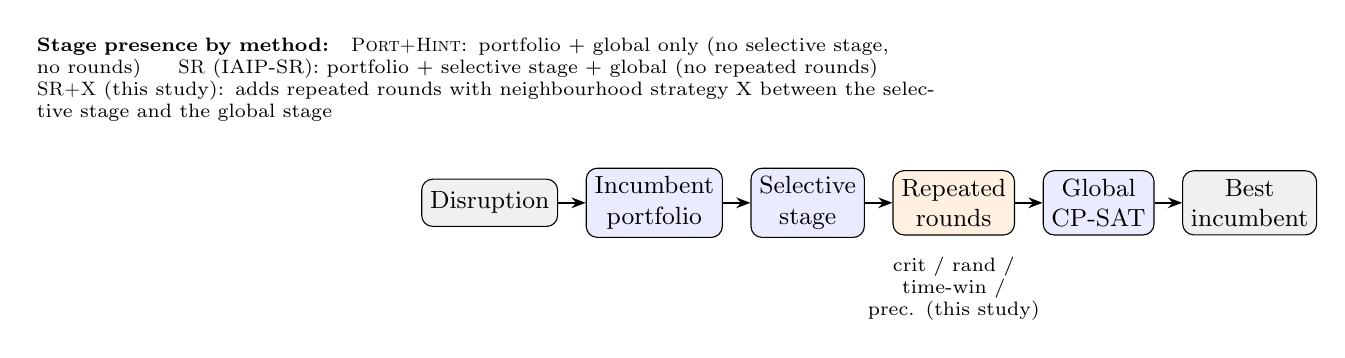
\begin{tikzpicture}[
  box/.style={draw, rounded corners, align=center, minimum height=0.6cm, font=\small, inner sep=3pt},
  arr/.style={-{Stealth[length=1.8mm]}, thick},
  node distance=0.35cm
]
\node[box, fill=gray!12] (dis) {Disruption};
\node[box, fill=blue!8, right=of dis] (port) {Incumbent\\portfolio};
\node[box, fill=blue!8, right=of port] (sel) {Selective\\stage};
\node[box, fill=orange!12, right=of sel] (rnd) {Repeated\\rounds};
\node[box, fill=blue!8, right=of rnd] (glob) {Global\\CP-SAT};
\node[box, fill=gray!12, right=of glob] (out) {Best\\incumbent};
\foreach \a/\b in {dis/port, port/sel, sel/rnd, rnd/glob, glob/out}
  \draw[arr] (\a) -- (\b);
\node[font=\scriptsize, below=0.15cm of rnd, align=center, text width=2.6cm]
  {crit / rand / time-win /\\ prec. (this study)};
\node[font=\scriptsize, above=0.6cm of dis, align=left, text width=11.5cm] (legend) {
  \textbf{Stage presence by method:}\quad
  \textsc{Port+Hint}: portfolio + global only (no selective stage, no rounds) $\quad$
  \textsc{SR} (IAIP-SR): portfolio + selective stage + global (no repeated rounds) $\quad$
  \textsc{SR+X} (this study): adds repeated rounds with neighbourhood strategy X between the selective stage and the global stage
};
\end{tikzpicture}
}
\caption{The unified pipeline and stage presence by method; $U(t)=\min\{C_{\max}(S): S$ a validated incumbent by time $t\}$.}
\label{fig:framework}
\end{figure*}

\begin{algorithm}[t]
\caption{One round of repeated restricted reoptimization}
\label{alg:round}
\begin{algorithmic}[1]
\REQUIRE incumbent $S$, disrupted operations $D$, targeting rule $\tau$, local deadline $T$
\STATE recompute $S$'s longest binding chains (calendar-aware: outages, releases, commitments)
\STATE build $N$ from $\tau$ (critical chain / random / time window / random precedence), seeded at $D$, $|N|$ matched across rules
\STATE $S' \gets$ CP-SAT solve of $N$'s restricted model, hinted with $S$, s.t.\ $C_{\max}\le U{-}1$
\IF{$S'$ strictly improves $S$}
  \STATE $S \gets S'$; repeat while time $<T$ remains
\ELSE
  \STATE stop (protocol M1) \textbf{or} continue to a fixed round count regardless (protocol M2)
\ENDIF
\end{algorithmic}
\end{algorithm}

One monotonic deadline covers the portfolio, every round, and the final unrestricted stage; every round's restricted model always contains the current incumbent as a feasible point, so the retained objective is non-increasing by construction --- an elementary property of the acceptance rule, not a per-round guarantee: a round may still fail, time out, or return a non-improving feasible schedule, and none of this is hidden or discarded (the certificate section below).

\section{Neighbourhood-Targeting Strategies (RQ3)}
\label{sec:lns}

Every control in Table~\ref{tab:methods} shares the identical initial incumbent, round policy, local window, global continuation and worker count as \crit{}, differing only in how each round's neighbourhood is chosen, so that any PI difference is attributable to neighbourhood \emph{content} rather than to a resource asymmetry. \tw{} and \precn{} are external, size-matched analogues of CP-SAT's own \texttt{Scheduling\-Time\-Window\-Neighborhood\-Generator} and \texttt{Random\-Precedence\-Scheduling\-Neighborhood\-Generator}.

\begin{table}[t]
\centering\footnotesize
\setlength{\tabcolsep}{2.3pt}
\begin{tabular}{lccccc}
\toprule
Method & Portf. & Select. & Rep. & Targeting & $w$ \\
\midrule
\base{} & Y & Y & N & critical chain & 1 \\
\crit{} & Y & Y & Y & critical chain & 1 \\
\rnd{} & Y & Y & Y & random ($|N|$-m.) & 1 \\
\tw{} & Y & Y & Y & time window ($|N|$-m.) & 1 \\
\precn{} & Y & Y & Y & random precedence & 1 \\
\ph{} & Y & N & N & -- (hinted only) & 1/4 \\
\native{} & Y & N & N & native LNS & 1 \\
\bottomrule
\end{tabular}
\caption{Method configuration: portfolio, single selective stage, repeated rounds, round targeting rule, worker count $w$ (\ph{} is run at both 1 and 4 workers; all repeated-round methods and \base{} use 1 worker).}
\label{tab:methods}
\end{table}

To separate the value of repetition (RQ2) from the value of targeting (RQ3), we run two protocols: \textbf{M1} (end-to-end) each method runs until the local window or a stop-on-failure condition, so round counts can differ between methods; \textbf{M2} (mechanism-isolation) every method is fixed to exactly 6 rounds of at most 0.4\,s each regardless of success, removing the confound that a method which more often finds nothing to improve simply finishes sooner.

For RQ4, \native{} is \ph{} run with \texttt{interleave\_search} on one worker, and \ph{} at four workers is CP-SAT's default multi-worker portfolio; both were verified from saved logs to activate all four internal scheduling LNS generators (\texttt{re\-sults/\-fi\-nal\_i\-caps/\-sol\-ver\_logs/}). We compare native search only at matched worker count, never across worker counts; at four workers (U3), the comparison uses $4\times$ the CPU-seconds of every one-worker setting by design, since U3 tests whether the external pipeline's advantage survives the solver's own parallel search, not whether CPU-seconds are held equal (a resource-normalized, equal-core-second variant was not run; see Discussion and Limitations).

\section{Correctness and the Certificate Result}
\label{sec:certificate}

The restriction machinery (kept-arc construction, the restricted model builder, the critical-chain computation) is reused unchanged from a prior stage, verified against two independent oracles (full enumeration and an independently-built CP-SAT model) on \OracleEnumCases\ and \OracleCpsatCases\ randomized cases with zero bound violations; for this study we additionally verified, on 250 randomized instances across all ten neighbourhood strategies with outages, release dates and commitments, that every restricted optimum lies between the full-problem optimum and the incumbent's value. A monotonic clock covers construction, every round, and the final stage; failed or non-improving rounds are recorded, not discarded; campaign resumption reproduces byte-identical output; 269 fast and 25 slow tests pass. A sound lower-bound \emph{certificate} for a restricted neighbourhood, verified against 5{,}500 independent oracle cases with zero violations, was decisive for only 13 of 200 restricted neighbourhoods tested; CP-SAT itself already proves the same non-improvement in a median of 21\,ms, and certificate-gated skipping, releasing, or budget allocation produced no measurable change in primal integral. We report this as a completed negative result.

\section{Experimental Methodology}
\label{sec:methodology}

\begin{table}[t]
\centering\small
\setlength{\tabcolsep}{3pt}
\begin{tabular}{ll}
\toprule
Parameter & Value \\
\midrule
Instance sizes & $m \times m$ full job shops, $m \in \{15,20\}$ \\
Durations & integer, uniform in $[5,50]$ \\
Deltas per stream & 10, weights 0.4/0.2/0.25/0.15 \\
 & (arrival/cancellation/duration/outage) \\
Solver & CP-SAT, OR-Tools 9.15, 1 worker \\
 & (4 in U3), $B=8$\,s (2/30\,s in U4/U5) \\
Development streams & seeds 301--310, 3 rounds, frozen \\
 & before any confirmatory run \\
Confirmatory streams & seeds 1101--1120 (40 $=$ 2 sizes \\
 & $\times$ 20 seeds), solver seeds 0--4 \\
Unit of inference & stream (base instance for U9) \\
Tests & exact sign test, Holm-corrected \\
 & within setting; bootstrap 95\% CI \\
 & (10{,}000 resamples), stream-clustered \\
Equivalence margin & $\pm10\%$ of comparator mean PI \\
 & (pre-registered, critical vs.\ time-window) \\
\bottomrule
\end{tabular}
\caption{Experimental configuration. Nine settings (U1 primary; U2 mechanism-isolation; U3 four workers; U4/U5 budget; U6/U7/U8 disruption-specific/severity; U9 34 published bases, Taillard/DMU/SWV/YN) run in fixed order on the held-out streams, confirmed unused elsewhere in this project's history.}
\label{tab:exp}
\end{table}

\paragraph{Criteria (fixed before the run).} C1: \crit\ beats \base\ by $\ge5\%$, CI upper $<0$, Holm $p<0.05$. C2: beats \rnd. C3: vs.\ \tw, classified superior/inferior/equivalent/inconclusive by the equivalence rule above. C4: beats \precn. C5: beats \native\ (1 worker). C6: beats \ph\ at 4 workers. \textbf{STRONG GO} requires C1--C6 all favourable; \textbf{CONDITIONAL GO} requires C1 and validity but allows C3 non-superior or C6 to fail; \textbf{NO-GO} if C1 fails or C3 is inferior.

\paragraph{Independent re-verification.} All 60{,}720 confirmatory runs were re-checked by a second analysis pipeline sharing no code with the one that produced the reported statistics. Every one of the 33 reported confirmatory comparisons reproduced to floating-point rounding (relative-difference error $<1.2\times10^{-16}$), with identical win/loss counts and Holm-adjusted $p$-values in every case (\texttt{re\-sults/\-fi\-nal\_i\-caps/\-ver\-i\-fied\_met\-rics.json}).

\section{Results}
\label{sec:results}

All \UOneRecords{} U1 and 60{,}720 total confirmatory runs returned a validated schedule (0 invalid, 0 unsolved).

\subsection{A. Repeated rounds vs.\ single-round and native search}

\begin{table}[t]
\centering\small
\setlength{\tabcolsep}{3pt}
\begin{tabular}{lrr}
\toprule
Method (U1, $n=\UOneN$) & mean PI & final gap \\
\midrule
\crit{} & \UOneMeanBTwocrit & \UOneGapBBTwocrit\% \\
\tw{} & \UOneMeanBThreetimewin & \UOneGapBBThreetimewin\% \\
\rnd{} & \UOneMeanBOnerandom & \UOneGapBBOnerandom\% \\
\precn{} & \UOneMeanBFourprec & \UOneGapBBFourprec\% \\
\base{} (IAIP-SR) & \UOneMeanBZeroiaip & \UOneGapBBZeroiaip\% \\
\ph{} & \UOneMeanBSixporthint & \UOneGapBBSixporthint\% \\
\native{} (1w) & \UOneMeanBFivenativeOnew & \UOneGapBBFivenativeOnew\% \\
\bottomrule
\end{tabular}
\caption{U1 absolute PI and final gap to $z^*$ by method (lower is better for both). Time-to-first-incumbent is $\approx$\UOneTfirstMsBTwocrit\,ms for every method, since it is dominated by the shared portfolio stage, not a differentiator. Figure~\ref{fig:forest} gives pairwise relative differences with CIs.}
\label{tab:main}
\end{table}

Table~\ref{tab:main} gives absolute PI; Figure~\ref{fig:forest} gives the six pairwise comparisons against \crit{} with 95\% CIs and significance. \textbf{C1, C2, C4 and C5 hold}: \crit{} beats \base{} (\UOneBTwocritVsBZeroiaipRel\%, Holm $p=\UOneBTwocritVsBZeroiaipHolm$), \rnd{} (\UOneBTwocritVsBOnerandomRel\%), \precn{} (\UOneBTwocritVsBFourprecRel\%) and \native{} (\UOneBTwocritVsBFivenativeOnewRel\%), while \rnd{} itself is not significantly better than \base{} ($\UOneBOnerandomVsBZeroiaipRel$\%): repeating the restricted stage with an \emph{unstructured} neighbourhood adds almost nothing by itself.

\begin{figure*}[t]
\centering
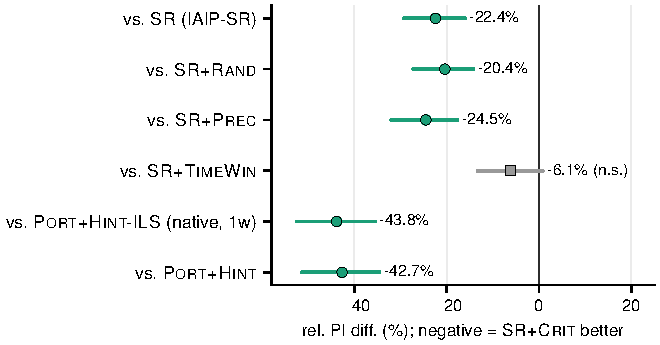
\includegraphics{figures/forest_u1.pdf}
\caption{U1 confirmatory: mean relative PI difference (\crit{} vs.\ each comparator) with 95\% bootstrap CI (stream-clustered, $n=\UOneN$); filled markers and solid CIs are significant (Holm $p<0.05$ and CI excludes zero), open squares are not. Recomputed directly from \texttt{confirmatory\_analysis.json}.}
\label{fig:forest}
\end{figure*}

\begin{figure}[t]
\centering
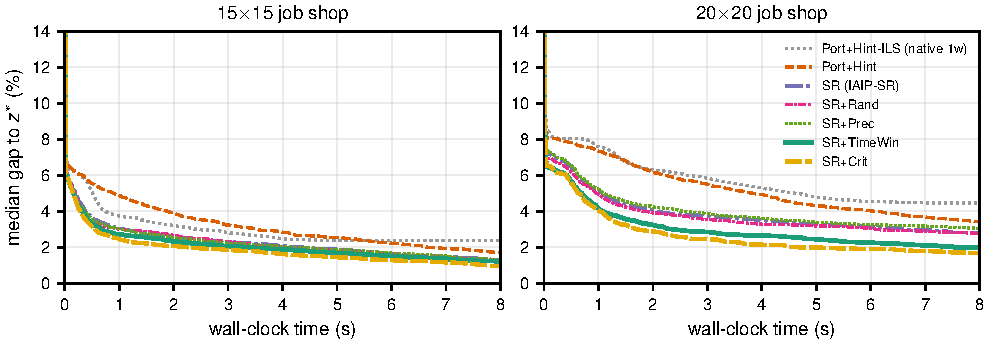
\includegraphics[width=\linewidth]{figures/trajectories.pdf}
\caption{Median gap to $z^*$ over time, U1 confirmatory streams (1{,}000 instance-step-seed combinations per size per method; real archived trajectories, not illustrative). At $B=8$\,s, \crit{} and \tw{} reach \FigTwoOneFiveCritAt\% / \FigTwoOneFiveTwAt\% ($15{\times}15$) and \FigTwoTwoZeroCritAt\% / \FigTwoTwoZeroTwAt\% ($20{\times}20$) median gap, both ahead of \base{} (\FigTwoOneFiveSrAt\% / \FigTwoTwoZeroSrAt\%).}
\label{fig:traj}
\end{figure}

\subsection{B. Does critical-region targeting beat time-window targeting?}
\label{sec:timewindow}

Figure~\ref{fig:mechanism} answers RQ3 directly and resolves an apparent exception by reanalysis of already-archived U1/U2/U6 raw trajectories; no new experiments were run. Panel A (end-to-end protocol, confirmatory) shows a significant critical-region advantage specifically after arrivals (U6) that is absent overall (U1) and after outages (U7). Panel B (matched-round protocol, M2) shows the \emph{opposite} sign overall: \crit{} is \UTwoMTwocritVsMTwotimewinRel\% \emph{worse} than \tw{} once round count is fixed (Holm $p=\UTwoMTwocritVsMTwotimewinHolm$), and the same reversal holds in every disruption type we broke the exploratory M2 grouping out by (arrival, cancellation, duration change, outage alike) --- those four points are exploratory (no pre-registered multiplicity correction, no separately-computed CI) and are drawn without error bars for that reason. Panel C shows why: under the end-to-end protocol, critical-region rounds complete systematically more rounds per instance than time-window rounds in every disruption type (e.g.\ arrival \RoundsUOneArrivalCrit{} vs.\ \RoundsUOneArrivalTw{} mean completed rounds), because critical-region rounds succeed more often per attempt and the stop-on-fail rule lets a method continue only after success --- more attempted rounds mean more chances to improve, independent of neighbourhood content. \textbf{We therefore do not claim critical targeting is better suited to any disruption type}; the apparent arrival exception is an artifact of unequal round counts, and this supersedes our own earlier reading of the same end-to-end data.

\begin{figure*}[t]
\centering
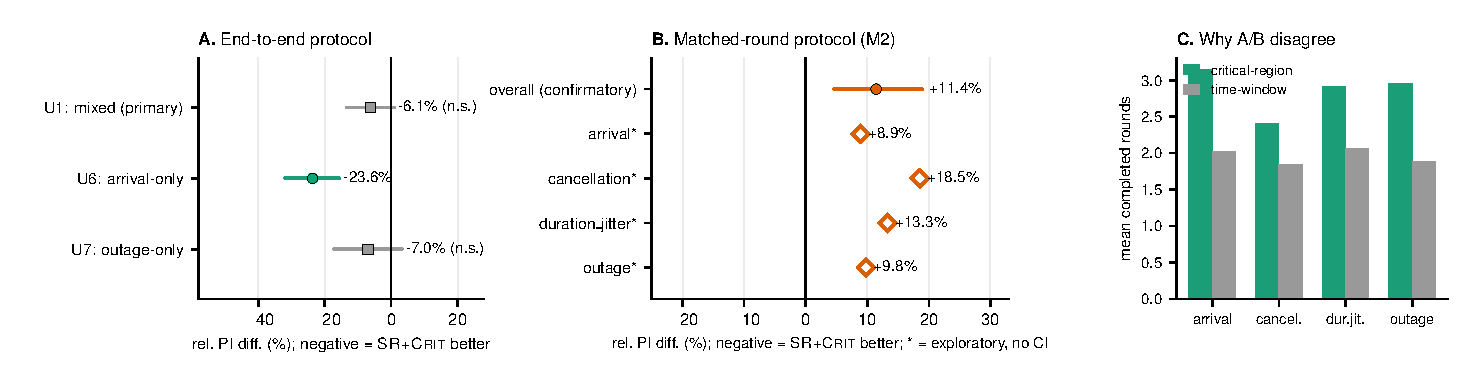
\includegraphics[width=0.78\linewidth]{figures/mechanism_u2_u1.pdf}
\caption{Critical-region vs.\ time-window targeting. \textbf{A}: end-to-end protocol (confirmatory, full CI), by setting. \textbf{B}: matched-round protocol (M2); overall is confirmatory with full CI, the four by-disruption-type points (*) are exploratory, transcribed from the already-published reanalysis, and carry no CI. \textbf{C}: mean completed rounds under the end-to-end protocol, the explanation for why A and B disagree. Negative = \crit{} better.}
\label{fig:mechanism}
\end{figure*}

A further reanalysis of U2's round-level metadata shows neighbourhood \emph{size} is matched almost exactly between critical and time-window rounds (\MTwoRoundCritN{} vs.\ \MTwoRoundTwN{} operations) but the resulting restricted subproblem's \emph{difficulty} is not: time-window rounds take \MTwoRoundTwVsCritPct\% longer to resolve on average (\MTwoRoundTwSolverS\,s vs.\ \MTwoRoundCritSolverS\,s) and more often exhaust their 0.4\,s cap without a definitive status (\MTwoRoundTwFeas\ vs.\ \MTwoRoundCritFeas\ rounds), while critical-region rounds more often resolve quickly to a proof of no improvement (\MTwoRoundCritInfeas\ vs.\ \MTwoRoundTwInfeas). Equal neighbourhood size does not imply equal search complexity.

\subsection{C. Native solver search and worker count (RQ4)}

\crit{} vs.\ \native{} (1 worker, confirmed from logs to run all four scheduling LNS generators on one thread): \UOneBTwocritVsBFivenativeOnewRel\% (Holm $p=\UOneBTwocritVsBFivenativeOnewHolm$) --- \textbf{C5 holds}. At four workers (U3, confirmed from logs to run the same four generators alongside three more), \crit{} vs.\ \ph{} is \UThreeBTwocritVsBSixporthintRel\% (Holm $p=\UThreeBTwocritVsBSixporthintHolm$) --- not significant; see the \textsc{4 workers} column of Figure~\ref{fig:heatmap}. \textbf{C6 fails}: with CP-SAT's own multi-worker scheduling LNS active, none of \base, \crit{} or \tw{} is distinguishable from the others.

\subsection{D. Robustness across budgets, severity and benchmarks (RQ6)}

\begin{figure*}[t]
\centering
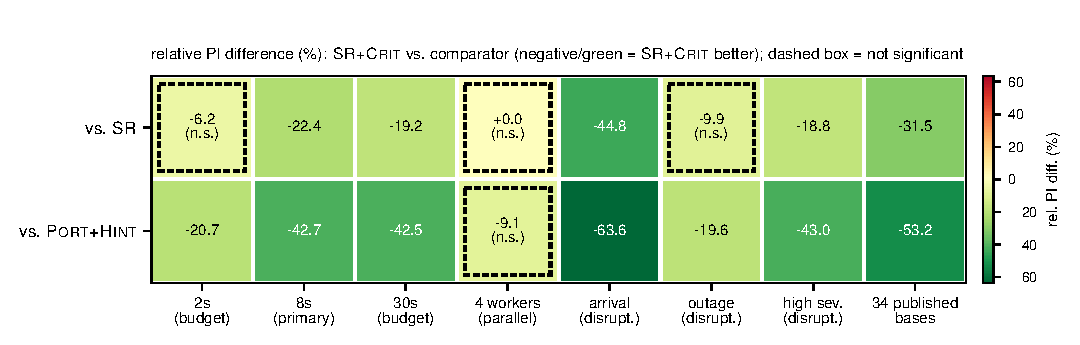
\includegraphics[width=0.97\linewidth]{figures/robustness_heatmap.pdf}
\caption{Relative PI difference, \crit{} vs.\ \base{} and vs.\ \ph{}, across every confirmatory setting. Dashed outline: not significant (Holm $p<0.05$ and CI excludes 0, both required). Recomputed directly from \texttt{confirmatory\_analysis.json}.}
\label{fig:heatmap}
\end{figure*}

Figure~\ref{fig:heatmap} consolidates U1 and U3--U9: the advantage over \base{} holds in every setting except the shortest budget (U4, 2\,s: \UFourBTwocritVsBZeroiaipRel\%, Holm $p=\UFourBTwocritVsBZeroiaipHolm$) and the four-worker setting, and is strongest on published benchmark bases (\UNineBTwocritVsBZeroiaipRel\%, U9). The advantage over \ph{} is larger and more consistently significant than the advantage over \base{} throughout, except again at four workers, where it also narrows sharply (U3: \UThreeBTwocritVsBSixporthintRel\%) relative to one worker (U1: \UOneBTwocritVsBSixporthintRel\%).

\section{Discussion and Limitations}
\label{sec:discussion}

Per our pre-registered classification, this is a \textbf{CONDITIONAL GO}: C1, C2, C4 and C5 hold reproducibly; C3 is not established as superior (and, after reanalysis, not even conditionally so after arrivals); C6 fails outright. Six findings follow, each with a practical consequence for a practitioner deploying this pipeline:

\begin{enumerate}
\item \textbf{Repeated restricted optimization helps.} Recomputing and re-solving a restricted neighbourhood several times, rather than once, substantially improves anytime quality over \base{} (Figure~\ref{fig:forest}). \emph{Consequence:} a single-round selective-repair pipeline is leaving quality on the table if the local time window has not yet closed.
\item \textbf{Structured targeting beats some random alternatives.} \crit{} beats \rnd{} and \precn{}, which are not themselves reliably better than \base{} (Table~\ref{tab:main}, Figure~\ref{fig:forest}). \emph{Consequence:} the neighbourhood must be spatially coherent, not merely repeated; an arbitrary or precedence-only relaxation is not a substitute.
\item \textbf{Critical-region targeting does NOT consistently beat time-window targeting, once rounds are matched.} Figure~\ref{fig:mechanism} shows the apparent arrival-specific exception is a round-count artifact, not a content effect. \emph{Consequence:} a practitioner may use the simpler, cheaper-to-compute time-window rule without a demonstrated quality cost.
\item \textbf{Round count/throughput materially matters.} Figure~\ref{fig:mechanism}C shows the same neighbourhood rule's apparent superiority can be entirely attributable to completing more rounds, not better content. \emph{Consequence:} any comparison of targeting rules that does not fix or report round counts risks this exact confound.
\item \textbf{More workers reduce the external pipeline's advantage.} Figure~\ref{fig:heatmap}'s \textsc{4 workers} column shows C6 fails: the gap over \ph{} narrows from \UOneBTwocritVsBSixporthintRel\% at one worker to \UThreeBTwocritVsBSixporthintRel\% at four. \emph{Consequence:} this pipeline's value is largest precisely where CP-SAT's own parallel search is most constrained (single-worker deployments).
\item \textbf{Strategy value depends on budget and disruption type.} Figure~\ref{fig:heatmap} shows the advantage is weakest at the shortest budget (U4) and strongest on published benchmark bases (U9); it is not a uniform multiplier. \emph{Consequence:} the pipeline's payoff should be re-measured for a deployment's actual budget and workload, not assumed from one setting.
\end{enumerate}

We do \emph{not} claim critical-region search is a superior targeting mechanism; the defensible claim is narrower (finding 3 above). Instances are synthetic full job shops from one generator; development and held-out streams share that generator. $z^*$ is the best value found in each setting, not a proven optimum. Only makespan is optimized; stability is not controlled. The C3 equivalence classification depends on a pre-specified $\pm10\%$ margin and a development-derived power estimate; non-significance under that margin is absence of demonstrated superiority, not proof of equivalence. CP-SAT's internal LNS generator selection is solver-version-specific; a different OR-Tools release could show different four-worker behaviour. U3's four-worker comparison uses $4\times$ the CPU-seconds of the one-worker settings by design (matched wall-clock, not matched core-seconds); a resource-normalized variant was not run and is left for future work, as is a scheduling-LNS-only native baseline. The full texts of \citet{sun2026} and \citet{linyang2026} remain inaccessible to us despite a renewed, documented attempt through legitimate routes.

\section{Conclusion}

Across a frozen, independently-reproduced confirmatory study, retaining a feasible incumbent and repeating a restricted CP-SAT stage with a recomputed, spatially-coherent neighbourhood reliably improves an anytime rescheduling pipeline over a single restricted stage, over unstructured repetition, and over the installed solver's single-thread scheduling search. Whether that coherent region should be the schedule's critical chain specifically, rather than a comparably simple time window, is not established by this evidence in any disruption type we tested once a round-count confound is removed; and the entire advantage over native search disappears once the solver is allowed to use its own multiple workers. We report the positive and the negative findings together, and the reanalysis that narrowed our own initial reading of the data, as the more defensible outcome of this investigation.

\bibliography{references}

\end{document}
